\documentclass[conference]{IEEEtran}
\usepackage{cite}
\usepackage{amsmath,amssymb}
\usepackage{booktabs}
\usepackage{url}
\usepackage{graphicx}
\usepackage{float}

\begin{document}

\title{Fact Cards Beside the Paragraphs:\\
A 20,000-Question Run on MechQA}

\author{
\IEEEauthorblockN{Krishna}
\IEEEauthorblockA{Department of Computer Science and Engineering\\
Sri Sairam Engineering College\\
Chennai, India}
\and
\IEEEauthorblockN{V. Saranya}
\IEEEauthorblockA{Department of Computer Science and Engineering\\
Sri Sairam Engineering College\\
Chennai, India}
}

\maketitle

\begin{abstract}
A materials question is usually after one number or one alloy name sitting inside a long paragraph. This paper asks whether handing the model a few short fact cards, on top of the nearest paragraphs, makes that answer easier to copy. The questions are 20{,}000 rows from the MechQA validation split. Paragraphs are ranked with \texttt{mxbai-embed-large} and cosine similarity. The generator is \texttt{Qwen3-8B-FP8} at temperature 0. The same instruction and the same cutoff of three are used for paragraphs alone, cards alone, and the combined prompt. Entity Lookup is finished: on 6{,}667 questions the combined prompt scores 0.015 exact match, cards alone 0.012, and paragraphs alone 0.005. The right paragraph is in the top three for only 1.6\% of those questions. Numeric Lookup is scored on 5{,}253 of 6{,}667 questions, where paragraphs (0.113) are just ahead of the combined prompt (0.111) and cards alone fall to 0.042. Property Identification is scored on 992 of 6{,}666 questions, where the combined prompt leads (0.167 against 0.149 and 0.043). These last two slices are still running. The combined prompt helps entity questions. It does not yet lead every question type.
\end{abstract}

\begin{IEEEkeywords}
retrieval-augmented generation, knowledge graph, mechanical properties, MechQA, exact match
\end{IEEEkeywords}

\section{Introduction}
Someone who already has the right paragraph can underline the number. The harder job is finding that paragraph. Papers on alloys repeat the same units, so a question about strength sits close to many different materials at once. A search that follows wording then brings back a paragraph on the right topic and the wrong alloy.

One way to keep a language model from inventing the number is to paste source text into the prompt \cite{lewis2020rag,guu2020realm,izacard2021fid,gao2023ragsurvey}. A model that is left to recall a fact from its parameters often misses or invents it \cite{petroni2019lama,ji2023hallucination,shuster2021hallucination}. The usual search ranks chunks by how close their embeddings are \cite{vaswani2017attention,devlin2019bert,reimers2019sbert,karpukhin2020dpr}. That works when the question already names the material, as in ``what is the yield strength of GNS/Cu.'' It slips when the question states the measurement and asks for the name, because lots of paragraphs carry a similar measurement and the right name need not be the nearest vector.

The same fact can be written as a short card: material, property, value. Search can then look for the value instead of for a paragraph that merely sounds related. The card is only as careful as the program that wrote it, and it leaves out the warnings that sit in the sentences around the number.

The proposed method builds both indexes from one locked set of paragraphs and compares two ways of filling the prompt. The first way sends the top paragraphs. The second way sends those paragraphs and then the top cards. The model, the instruction, the temperature, and the cutoff are the same, so a change in score comes from what was pasted in. A third run drops the paragraphs and keeps the cards. That run is reported so the combined score is not read as the winner. It is not a third screen in a product.

The questions come from MechQA \cite{zhang2026mechqa}. Each row has a question, one source paragraph, and a short recorded answer. The people who released that file score a reader who is already holding the right paragraph. This study withholds that paragraph and requires the system to find it. This is not the textbook question set in ManuRAG \cite{li2026manurag}, and the percentages printed there are not a target for the present experiment.

The contribution of this paper is a comparison, fixed before any answer was scored, of paragraphs alone against the same paragraphs plus cards. The 20{,}000 validation questions are broken out by question type. The comparison also counts how often the right paragraph is among the top three. A split by the five mechanical properties is held until Numeric Lookup and Property Identification have been scored in full, so a half-finished slice is not averaged in as if it were the sample.

\section{Related Work}
\subsection{Passage retrieval and generation}
Lewis and colleagues pull passages by dense similarity and then let a sequence model read the question glued to those passages \cite{lewis2020rag}. The model may copy a span or write a new sentence. Early open-domain systems already retrieved Wikipedia passages before reading them \cite{chen2017drqa}. Later retrievers train a question encoder and a passage encoder so the right passage ranks above others from the same collection \cite{karpukhin2020dpr,xiong2021ance,khattab2020colbert}. Generative readers then condition on those passages, either by pre-training with a retrieval step or by fusing the top passages at generation time \cite{guu2020realm,izacard2021fid,izacard2023atlas,borgeaud2022retro}. In all of those designs the thing you retrieve is still a passage. None of them keeps the measurement as its own object, ready to be matched when the question and the paragraph use different words.

That gap shows up quickly in technical writing. Ask about 851~MPa and every paragraph that mentions a tensile strength near that size looks alike. The embedding piles those paragraphs together. The alloy name, which is the actual answer, is only a small piece of the vector. Sorting by the whole paragraph then prefers ``this is about strength'' over ``this is the exact value.''

\subsection{Graphs over a corpus}
A knowledge graph is a set of entities joined by typed edges \cite{hogan2021kg}. Joining that store to a language model is surveyed as its own research line \cite{pan2024llmkg}. One design scores paths on the graph before the model answers \cite{yasunaga2021qagnn}. Edge and colleagues pull entities and relations out of a corpus, write summaries of groups in the graph, and answer from those summaries rather than from the nearest chunks alone \cite{edge2024graphrag}. Their target is a written briefing over a document collection. The graph there is a way to summarise. The graph in the present study is smaller. Each card is one mechanical-property fact, and the reply has to be a short string that matches a recorded answer. Community summaries are not built. The graph is a list of \((m,p,v)\) rows with a pointer back to the paragraph they came from.

Other combined systems fetch passages and then add neighbours from a graph. The neighbour helps when it supplies a fact the passage never stated. It hurts when the passage is already the wrong one and stays in the prompt, because the model treats every line it was given as fair evidence. The present experiment is that second case, and the counts below are arranged to show it.

\subsection{Manufacturing questions and MechQA}
ManuRAG lines up textbook prose with descriptions of figures and tables before it embeds them, and it tests questions drawn from a manufacturing textbook \cite{li2026manurag}. What gets retrieved is still mixed text and pictures. A graph of equipment, work orders, and standards is not part of that design. Their scores belong to a closed question file and a different model. That work is cited because manufacturing questions are the wider problem, not because the present experiment tries to match those percentages.

Embeddings of the materials literature already place related compounds near one another \cite{tshitoyan2019nature}. Domain language models and extraction pipelines have been built for that literature \cite{gupta2022matscibert,olivetti2020apr,weston2019ner}. MechQA is drawn from mechanical properties already tabulated in the literature \cite{zhang2026mechqa}. The public file holds 202{,}068 rows laid out like SQuAD: a question, a context paragraph, and an answer span with a character offset. Each row is tagged with one of three question types. Numeric Lookup asks for a value. Entity Lookup asks which material has a stated value. Property Identification asks which property a stated value belongs to. The original tests hand the right paragraph to the reader and score extraction. Once the paragraph is given, the search problem studied here disappears. This study indexes the paragraphs and requires the system to locate the useful one.

\section{Problem Setup}
Call the corpus a set of paragraphs \(\{d_1,\ldots,d_N\}\) and call the question \(q\). The retrieved text is packed into a string \(c\). A generator \(G\), always at temperature 0, writes
\begin{equation}
\hat{y} = G(q, c).
\end{equation}
The recorded answer \(y\) is a span inside one source paragraph. The whole of \(\hat{y}\) is not scored. The instruction tells the model to finish with a line that starts \texttt{Result:}, and only the words after that marker are compared. Otherwise a long explanation would be matched, character for character, against a short span.

The comparison is SQuAD exact match \cite{rajpurkar2016squad,rajpurkar2018squad2}. Both strings are lowercased. Punctuation is stripped. The words \(a\), \(an\), and \(the\) are stripped. What remains must be the same string. A reply that has the right span plus a unit note, a second number, or another name for the alloy is still wrong. The rule was kept tight so the three setups can be compared on one scale. It also explains misses a person would have let through. Those near misses are counted on their own in Section~\ref{sec:results}. They are not folded into the exact-match table.

The sample has three kinds of question. Numeric Lookup asks for a value, for example ``What is the yield strength of GNS/Cu?'' Entity Lookup asks for a material given a value, for example ``Which compound has an ultimate tensile strength of 851~MPa?'' Property Identification asks which recorded property a value belongs to. The properties that actually show up are yield strength, ultimate tensile strength, fracture strength, Young's modulus, and ductility. Fracture strength has 510 questions in the sample. Its exact-match rate is not printed until the unfinished question types are complete.

The operating modes differ only in \(c\):
\begin{align}
c &= c_V && \text{vector}, \\
c &= c_G && \text{graph only}, \\
c &= c_V \,\|\, c_G && \text{hybrid}.
\end{align}
The symbol \(\|\) means concatenation. Paragraphs are written first. Triples are written second, under the heading used by the pilot program. No other text is inserted.

\section{Method}
\subsection{Vector retrieval}
The same embedding model turns each paragraph \(d\) and the question \(q\) into vectors \(\mathbf{v}_d\) and \(\mathbf{v}_q\). Order is cosine similarity, the comparison used by the vector-space model of documents \cite{salton1975vsm,manning2008ir},
\begin{equation}
s(q,d) = \frac{\mathbf{v}_q \cdot \mathbf{v}_d}{\|\mathbf{v}_q\|\,\|\mathbf{v}_d\|}.
\end{equation}
The paragraph context \(c_V\) is the text of the \(k\) paragraphs with the biggest \(s(q,d)\). Here \(k=3\). Paragraphs are embedded as search documents. The question is embedded as a search query. Those vectors are computed once and saved. Later runs do not embed the corpus again.

Each paragraph goes into the prompt as one line: a short id, the DOI of the article, and the paragraph itself. The id is there so the later analysis can check whether the right paragraph was in the three. The model is not asked to print it.

\subsection{Graph construction}
From each paragraph an extractor writes triples
\begin{equation}
(m, p, v),
\end{equation}
with \(m\) a material, \(p\) a property name, and \(v\) the value on the page, plus the id of the paragraph it came from. This run keeps 1{,}389 triples from 4{,}144 paragraphs. The extractor may skip a fact or glue a value to a shortened alloy name. Those mistakes were left in. Fixing them by hand would describe a cleaned store, not the pipeline that actually ran.

A question is tied to a triple by shared words, not by another embedding. The score is a raw overlap count, not a BM25 weight \cite{robertson2009bm25}. The proposed method takes question tokens longer than two characters. A triple scores how many of those tokens show up in \(m\), \(p\), or \(v\). The card context \(c_G\) is the \(k\) triples with the highest score, written as
\begin{equation}
m \xrightarrow{\text{has\_property}} p \xrightarrow{\text{has\_value}} v.
\end{equation}
Ties stay in sort order. Nothing learns a rank over the cards. The proposed method uses the same \(k=3\) as on the paragraph side, so the combined prompt is not given a longer list of facts than of paragraphs.

Word overlap likes questions that already contain the alloy or the property. ``Yield strength'' together with ``GNS/Cu'' hits a card that contains those strings. A question that only has ``851'' and ``MPa'' hits every card whose value contains those tokens, and the top three are whichever of those cards share the most leftover words. Cutting at three does not promise that the true material is first.

\subsection{Hybrid retrieval}
The combined setup does not first decide what kind of question it has. It always builds
\begin{equation}
c_H = c_V \,\|\, c_G.
\end{equation}
There is no learned reranker \cite{nogueira2019bert}, and there is no rule that throws out a paragraph when its cosine score is weak. If the three paragraphs are the wrong ones, they still sit in the prompt next to the cards. The model is told to use only what it was given. It is not told to trust the cards when they disagree with the paragraphs. That clash is left to the model at temperature 0. The reply will be the same if the call is repeated. It will not necessarily match the recorded span.

\subsection{Prompt and decoding}
Every setup and every question gets the same instruction:
\begin{quote}
\small
Answer the question using only the context below. If the context is insufficient, say so. End with the line: \texttt{Result:} followed by a short answer.
\end{quote}
The context block and the question come after that. The experiments request one completion per question per setup. Temperature is 0. There is no extra system prompt and no worked example in front. The three setups cannot differ because the instruction was worded differently. They differ because different lines were placed in the context block.

\subsection{What this pilot leaves out}
A separate industrial copilot, not scored here, fetches approved document chunks by cosine distance and then adds graph edges that belong to those documents. In that design the graph does not search by itself. Miss the document in the vector step and the edges from the right document never load. On MechQA the proposed method searches the card list directly, including when the right paragraph is outside the top three. Both ideas paste two sources into one prompt. The way the sources are chosen is not the same, and screenshots of that copilot are not evidence for the table in Section~\ref{sec:results}.

The study also did not train a router that decides when retrieval is needed \cite{asai2024selfrag}, did not build a tree of paragraph summaries \cite{sarthi2024raptor}, did not drop low-scoring paragraphs, and did not fine-tune the generator on MechQA. The training split of the file was never read.

\section{System Architecture and Implementation}
Figure~\ref{fig:arch} is the path from one question to a scored line. The question is embedded and also matched against the fact cards. Paragraphs-only keeps the three nearest paragraphs. Cards-only keeps the three best cards. The combined prompt keeps the paragraphs and then the cards. All three setups call the same generator at temperature 0. The recorded answer is used only after the \texttt{Result:} line is written.

\begin{figure}[H]
\centering
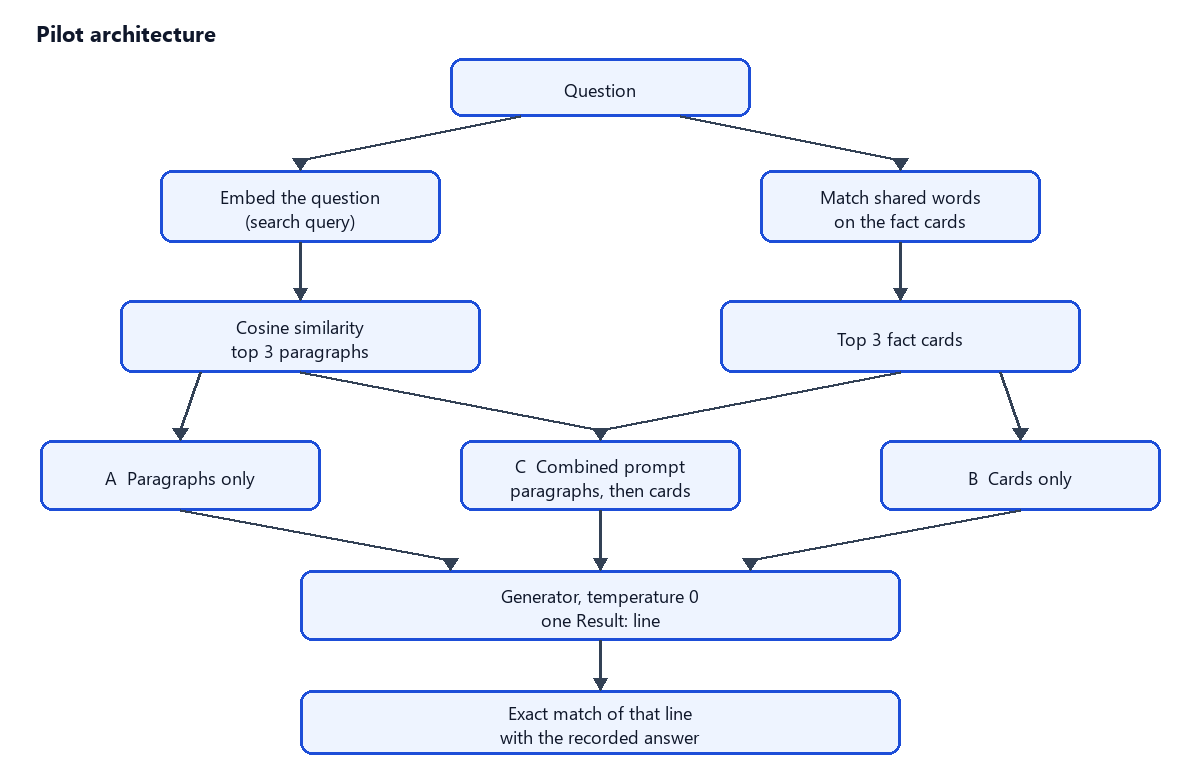
\includegraphics[width=\columnwidth]{figures/architecture.png}
\caption{Architecture of the pilot. Condition C places the fact cards after the paragraphs. Conditions A and B each keep one of those two lists.}
\label{fig:arch}
\end{figure}

Figure~\ref{fig:code} is the code that builds that prompt. \texttt{format\_context} writes the paragraphs first and, when cards are requested, appends them under the heading \texttt{Graph facts:}. The loop maps condition A to paragraphs only, condition B to cards only, and condition C to both. The same function fills the context string for every condition, so the instruction does not change.

\begin{figure}[H]
\centering
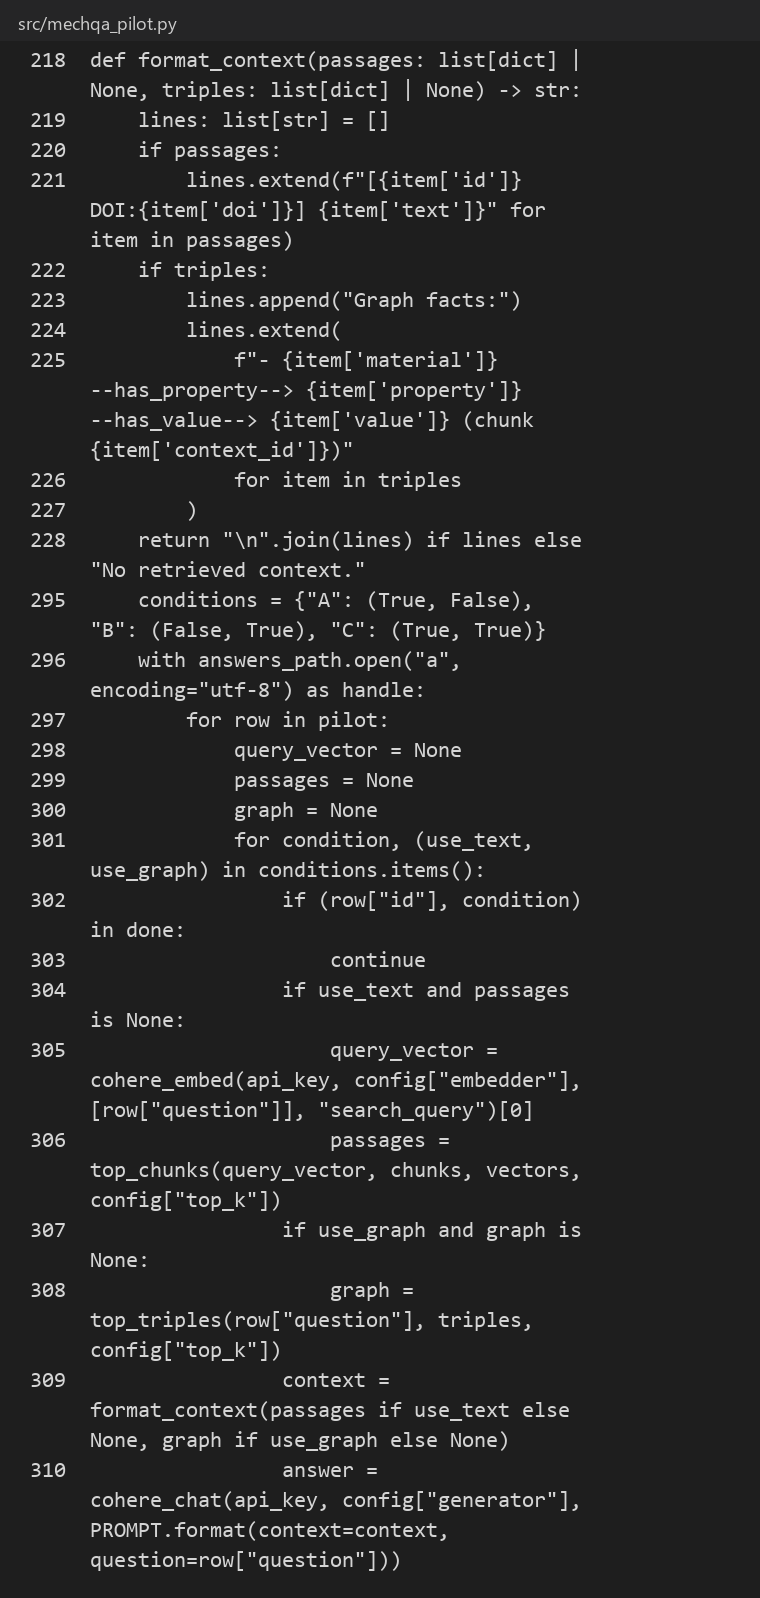
\includegraphics[width=\columnwidth]{figures/code_context.png}
\caption{Excerpt from \texttt{src/mechqa\_pilot.py}. The combined condition passes both the retrieved paragraphs and the retrieved cards into one context string.}
\label{fig:code}
\end{figure}

\section{Data}
MechQA holds 202{,}068 rows. The authors mark 20{,}346 of them as validation, and that is the only split opened for this study. Inside it the experiments used 20{,}000 rows. Within each question type the rows were sorted by the SHA-256 hash of the row id and a quota was kept from the front of that order: 6{,}667 Entity Lookup, 6{,}667 Numeric Lookup, and 6{,}666 Property Identification. Sorting by hash means the sample does not depend on the order of lines in the download. The quotas were chosen before the first scored call.

Those 20{,}000 questions sit in 4{,}144 different paragraphs. The search index is exactly those 4{,}144 paragraphs. It is not the training split, and it leaves out the 346 validation rows that were not drawn. The right paragraph is in the index. It reaches the prompt only if cosine similarity puts it in the top three. The system can still miss by fetching the wrong neighbours, even though the answer text is sitting in the index.

Some recorded spans in the public file do not match the property named in the question, and some cards shorten an alloy name that the recorded span writes in full. Those rows were retained. Dropping them after seeing the scores would let the result edit the sample. They stay in the denominator of every rate, as noise in the file.

Table~\ref{tab:sample} shows how the 20{,}000 questions spread across properties. Ultimate tensile strength and yield strength make up most of the sample. Fracture strength has 510 rows. That count is the sample, not a score.

\begin{table}[t]
\caption{The 20{,}000 questions by recorded property. The quotas were applied on question type, so the property counts are whatever the hash sample produced.}
\label{tab:sample}
\centering
\begin{tabular}{lr}
\toprule
Property & Questions \\
\midrule
Ultimate tensile strength & 8{,}194 \\
Yield strength & 7{,}017 \\
Ductility & 2{,}289 \\
Young's modulus & 1{,}990 \\
Fracture strength & 510 \\
\midrule
All properties & 20{,}000 \\
\bottomrule
\end{tabular}
\end{table}

\section{One Question, Start to Finish}
Every question goes through the same steps. They are written here on the GNS/Cu question so a reader can follow one pass without opening the program.

\begin{enumerate}
\item Read the question from the locked sample: ``What is the yield strength of GNS/Cu?'' The span stored beside it is 542~MPa. That span is never shown to the model.
\item Embed the question as a search query. Each of the 4{,}144 paragraphs already has a stored document vector. Cosine similarity orders the paragraphs. Keep the top three, even when the third is only a hair above the fourth.
\item Also match the question to the 1{,}389 cards by shared words. Tokens shorter than three characters are ignored, so a unit or a single letter does not run the score. Keep the top three cards.
\item Paragraphs-only builds a prompt from the instruction, the three paragraphs, and the question. The combined setup uses that prompt and adds the three cards under a short heading. Cards-only uses the instruction and the three cards, with no paragraphs.
\item The model returns one completion at temperature 0. The scorer takes the last \texttt{Result:} line. On this question the paragraphs-only line is ``542 MPa (tensile), 637 MPa (compressive).'' The combined line is ``542 MPa.''
\item Exact match cleans both the recorded span and that line: lowercase, punctuation gone, articles gone. ``542 MPa'' matches. The longer line does not, because the extra words are still there after cleaning. Paragraphs-only is a miss that still contains the right number. The combined reply is a hit.
\end{enumerate}

None of the steps look at the recorded span before the reply is written. That span is used only in the last step. The boxes later in the paper are steps four and five for this one question. The tables in Section~\ref{sec:results} count that last step on the rows scored so far. The boxes in the next section are a walk-through from an earlier 200-question pass with a different generator. They show the prompt shape. They are not rows from Table~\ref{tab:em}.

The word score in step three is easy to write down. Let \(T(q)\) be the question tokens longer than two characters, and let \(T(m,p,v)\) be the tokens in the material, the property, and the value. The rank key is how big the overlap is,
\begin{equation}
r(q, m, p, v) = \lvert T(q) \cap T(m, p, v) \rvert.
\end{equation}
A card with \(r=0\) stays out of the prompt. If fewer than three cards score above zero, only those are pasted in. The rank key does not know which token is the alloy and which is the unit. On an entity question the shared tokens are often the number and the property name, so several alloys with that property compete, and cutting at three is an arbitrary cut among them.

\section{Experimental Setup}
The generator is \texttt{Qwen/Qwen3-8B-FP8} at temperature 0, served with vLLM 0.31.0 from this project's own environment. Thinking is switched off. Embeddings are \texttt{mxbai-embed-large}. Each setup is one call per question, so the full sample is 60{,}000 generations. The sample file, the paragraph file, and the embedding file were written before that loop. Cards were extracted from the 4{,}144 paragraphs before answer scoring. If a call failed, the run picked up from the question-and-setup pairs already saved. If the answer file has a duplicate line, the last record for that pair is the one retained.

Entity Lookup has all 6{,}667 questions under all three setups. Numeric Lookup has 5{,}253 of 6{,}667, and Property Identification has 992 of 6{,}666. Those two slices were still being generated when the table was written. The rates below use only the finished rows in each slice. They are not filled in with zeros for the rows that have not been called yet.

Cards-only uses \(c_G\) and no paragraph text. It is a check, not a product mode. It asks whether the cards, with nothing else, are enough. It is reported so a lift of the combined prompt over paragraphs alone is not read as ``the merged prompt won all three runs.''

\section{What the Model Actually Saw}
This MechQA run has no application screen. Both setups are batch calls. The boxes here are the context that was sent, written out so a reader can see the difference without opening a log. They use one real numeric question: ``What is the yield strength of GNS/Cu?'' The recorded answer is 542~MPa. A later box uses an entity question that all three setups miss, so the picture is not only a success.

\begin{figure}[H]
\centering
\fbox{\begin{minipage}{0.94\columnwidth}
\small
\textbf{Paragraphs only: follow similar wording.}\\[0.35em]
The question is set against every paragraph. The three that sound most like it go to the model. Nothing else is added.\\[0.35em]
On this question those paragraphs were: one on a graphene--copper material (GNS/Cu), one on a solder alloy, and one on a titanium composite. The model read the first and wrote\\
\texttt{Result: 542 MPa (tensile), 637 MPa (compressive).}\\[0.35em]
542~MPa is in that line. The scored line has to be exactly ``542 MPa,'' so the longer line is marked wrong.
\end{minipage}}
\caption{Paragraphs-only example for ``What is the yield strength of GNS/Cu?'' The model sees only the three closest paragraphs.}
\label{fig:ui-vector}
\end{figure}

\begin{figure}[H]
\centering
\fbox{\begin{minipage}{0.94\columnwidth}
\small
\textbf{Combined: those paragraphs, then three fact cards.}\\[0.35em]
The combined prompt keeps the three paragraphs above and adds the three best short facts:\\
GNS/Cu composite --- yield strength --- 542~MPa\\
TNTZ-2Fe-0.4O --- yield strength --- 817~MPa\\
longitudinal reinforcement --- yield strength --- 553~MPa\\[0.35em]
The model can read the card instead of digging through the paragraphs. It wrote\\
\texttt{Result: 542 MPa.}\\[0.35em]
That line matches the recorded answer. The other two cards stay in the prompt. They are not taken out.
\end{minipage}}
\caption{Combined example for the same GNS/Cu question. The cards are added after the paragraphs. They do not replace them.}
\label{fig:ui-hybrid}
\end{figure}

The two boxes are one question, not the score. Here the paragraph search did fetch the right paragraph. Exact match still failed because the reply named two strengths. The combined prompt had those same paragraphs plus a card with a single number, and the reply matched. Section~\ref{sec:results} shows that a helpful card beside a noisy paragraph is not what happens on every question type.

\section{Results}
\label{sec:results}
\subsection{Exact match by question type}
Table~\ref{tab:em} is exact match on the rows scored when this section was written. Entity Lookup is complete. The other two rows are partial, and the denominator is the number already scored, not the quota. No overall line is printed. Averaging a finished slice with two unfinished slices would look like a result for all 20{,}000 questions.

On Entity Lookup the combined prompt is the best of the three: 98 of 6{,}667 (0.015), against 78 for cards alone (0.012) and 34 for paragraphs (0.005). On the 5{,}253 numeric questions scored so far, paragraphs lead by a small margin, 596 (0.113) against 584 for the combined prompt (0.111). Cards alone are right on 218 (0.042). On the 992 property questions scored so far, the combined prompt leads, 166 (0.167) against 148 for paragraphs (0.149) and 43 for cards (0.043).

\begin{table}[t]
\caption{Exact match on the MechQA rows scored so far. Entity Lookup is complete. The other two rows are still running, and the count in parentheses is the number scored.}
\label{tab:em}
\centering
\begin{tabular}{lccc}
\toprule
Question type & Paragraphs & Combined & Cards only \\
\midrule
Entity Lookup (6{,}667) & 0.005 & 0.015 & 0.012 \\
Numeric Lookup (5{,}253 of 6{,}667) & 0.113 & 0.111 & 0.042 \\
Property Identification (992 of 6{,}666) & 0.149 & 0.167 & 0.043 \\
\bottomrule
\end{tabular}
\end{table}

On the finished entity slice, both paragraphs and the combined prompt are right on 17 questions. The combined prompt alone is right on 81. Paragraphs alone are right on 17. Neither is right on 6{,}552. The gain is those 81 minus those 17. On the numeric rows scored so far the two setups trade places: the combined prompt alone is right on 143, and paragraphs alone are right on 155. On the property rows scored so far the combined prompt alone is right on 56, and paragraphs alone are right on 38.

\subsection{Was the right paragraph in the three?}
Paragraph search puts the right paragraph in the top three for 2{,}042 of 5{,}253 Numeric Lookup questions (38.9\%), 345 of 992 Property Identification questions (34.8\%), and 109 of 6{,}667 Entity Lookup questions (1.6\%). The combined setup uses those same three paragraphs, so it has the same hit rate on each slice. Cards-only has no paragraph list, so a hit rate is not defined for it.

Entity questions share numbers across many paragraphs. Inside an index of 4{,}144 paragraphs the nearest one is usually a different alloy. The card list keeps the number next to a material name, which is why cards alone and the combined prompt both clear paragraphs on that type. Unlike the earlier 200-question pass, the combined prompt does not fall below cards alone here. It is still a low rate: 98 hits in 6{,}667 questions.

On the property rows scored so far the right paragraph is present about one time in three, not three times in four. Paragraphs are no longer the best of the three on that partial slice. Cards alone stay far behind, so the lift is not ``cards instead of paragraphs.'' It is paragraphs plus a few cards.

\subsection{Exact match by property}
A split of exact match by yield strength, ultimate tensile strength, ductility, Young's modulus, and fracture strength is not reported. Numeric Lookup and Property Identification are unfinished, and the rows scored so far are not a balanced draw of those properties. Table~\ref{tab:sample} is only the composition of the locked 20{,}000. It is not a score.

\subsection{The right words, still a miss}
Exact match throws out a line that contains the recorded string and then adds words. That near-miss count was made on the earlier 200-question pass. It has not been repeated on these 20{,}000 questions, so the old counts of 22 and 54 are not carried forward.

\subsection{An entity question all three miss}
The GNS/Cu boxes are a case where the card helps. The next question is a case where the card has the wrong name. The question is ``Which compound has a ultimate tensile strength of 851~MPa?'' The recorded span is TNTZ-2Fe-0.4O. The top paragraphs do not include the right paragraph. The paragraphs-only reply says 851~MPa is not in the context. The top cards include ``TNT-Fe-O --- ultimate tensile strength --- 851~MPa,'' plus two other alloys at 1130~MPa and 1000~MPa. Cards-only and the combined prompt both answer TNT-Fe-O. Exact match marks both wrong. The transcript is from the earlier pass. It is kept because it shows the failure mode behind the entity column, not because those three replies were regenerated with \texttt{Qwen3-8B-FP8}.

\begin{figure}[H]
\centering
\fbox{\begin{minipage}{0.94\columnwidth}
\small
\textbf{What this miss is showing.}\\[0.35em]
Paragraphs-only had no paragraph that stated 851~MPa, so it refused. The card list had 851~MPa stuck to a shortened name, TNT-Fe-O, not to the recorded span TNTZ-2Fe-0.4O. The combined prompt kept the unhelpful paragraphs and the shortened card, and it copied the card.\\[0.35em]
A fact card is only as good as the name written on it. Pasting the card next to the paragraphs does not check that name against the recorded span.
\end{minipage}}
\caption{Entity-lookup miss on 851~MPa. The combined prompt followed the card, and the card did not use the recorded name.}
\label{fig:entity-miss}
\end{figure}

This one row is not a rate. It is what sits behind the entity column of Table~\ref{tab:em}. The value matches. The string exact match wants does not. Some of those clashes are extraction mistakes. Some are recorded spans a person would call the same as the extracted name. The study does not separate those two causes.

\section{Discussion}
The index is 4{,}144 paragraphs, so a top-three list is a much thinner cut than it was on the 192-paragraph pilot. That is why every exact-match rate in Table~\ref{tab:em} sits far below the rates from that pilot. The ordering is also not the same, and the unfinished slices can still move.

Entity lookup is the clearest finished picture. The right paragraph is in the top three for 109 of 6{,}667 questions. Paragraphs alone are right 34 times. Cards alone are right 78 times. The combined prompt is right 98 times. Adding the cards helps, and on this slice the paragraphs left in the prompt do not pull the combined score back under cards alone. Most entity questions are still misses for every setup, because neither list usually holds the recorded name.

Numeric lookup, on 5{,}253 questions, is the opposite small gap. Paragraphs are right 596 times and the combined prompt 584 times. Cards alone are right 218 times. The paragraphs are doing the work. The cards, by themselves, are not. Property identification is only 992 questions so far. There the combined prompt leads (166 against 148 and 43), and the right paragraph is present about 35\% of the time. That is not the pattern from the pilot, where paragraphs won that type. It is also not a finished count.

Two changes were not in this run. A router could send entity questions to the cards and numeric questions to the paragraphs. That router's score is not claimed, because the rule would be picked after seeing Table~\ref{tab:em}. Another change would drop paragraphs below a similarity cutoff before merging. Neither change was tested. Until Numeric Lookup and Property Identification finish, the claim that holds is the finished slice: on 6{,}667 entity questions, adding cards to the top paragraphs beats both paragraphs alone and cards alone, and the absolute rate stays under 0.02 because the right paragraph is rarely retrieved.

\section{How to Read a Miss}
A miss in the table is not one kind of mistake. Four patterns cover the replies inspected while the rates were counted. Naming them does not change a rate. It says what the rate is mixing.

The first pattern is a refusal. The \texttt{Result:} line says the context does not contain the answer. That is the honest line when the top paragraphs and the top cards really do not state the fact. On entity lookup, paragraphs-only often lands here, because the right paragraph is outside the top three and no card is supplied. Calling the refusal a miss is correct under exact match. It also shows that the search, not the model, dropped the fact.

The second pattern is a longer true line. The recorded string sits inside the \texttt{Result:} line, and extra words keep the strings from matching after cleaning. The paragraphs-only reply on GNS/Cu is this pattern. How often it happens on the 20{,}000-question run has not been counted. The combined prompt can produce it when a card and a paragraph give the model two ways to say one number, and the model keeps both. Exact match then marks down the fuller sentence.

The third pattern is a wrong neighbour. The reply names a real material and a real value from the context, and they are not the recorded pair. The 851~MPa reply TNT-Fe-O is this pattern when the card itself has the wrong name, and it is also this pattern when the card is right and the model copies a different card from the same list of three. The prompt always offers three cards. Nothing marks which of the three should be copied.

The fourth pattern is a recorded span a person might accept under different words. A shortened alloy name, a value written once as a percent and once as a fraction, or a property described in a sentence rather than by the label in the question, all fail exact match. Those rows are not relabeled. Doing that after reading the replies would let the scorer chase the model. The public span stays the span.

The boxes are a key to the kind of miss, not a second score. If a boxed reply has the recorded number and then extra words, it is the second pattern and it is still a miss in Table~\ref{tab:em}. If a boxed reply copies a card whose name is not the recorded name, it is the third pattern and it is a miss for both the combined prompt and cards-only. The rates in that table are what is left after all four patterns have been marked wrong.

\section{Limits of This Pilot}
Entity Lookup is one finished sample of 6{,}667 rows, one model, and one embedding. Confidence intervals are not reported. Numeric Lookup and Property Identification in Table~\ref{tab:em} are incomplete. A later page should replace those two rows when their quotas are full, rather than treat 0.113 and 0.167 as final. Ultimate tensile strength alone has 8{,}194 of the 20{,}000 questions, so a property split can still move the average once it is computed on the finished file.

The index is the 4{,}144 paragraphs that belong to the sampled questions. A search over all 20{,}346 validation paragraphs would meet more look-alike alloys. The hit rates above are therefore easier than a search of the full collection. They still show entity lookup failing inside this index: the right paragraph is retrieved 109 times in 6{,}667.

Noise in the recorded spans puts a ceiling on exact match that is not separated from search error. The 851~MPa row is the kind of row that feeds that ceiling. Diagrams, pump logs, and a person correcting edges are not in MechQA, and they are not claimed. The industrial copilot mentioned earlier chooses its sources differently and was not scored on these 20{,}000 questions.

Card ranking uses shared words, not a trained retriever. A dense ranker over cards might put the 851~MPa card behind a card whose material string matches the recorded span, or it might not. That comparison was not run. The model was not fine-tuned. A model trained to copy the shortest matching card would change both the exact-match rate and the near-miss rate. Temperature 0 takes away sampling noise. It does not take away a clash between a paragraph and a card.

\section{Conclusion}
On the finished Entity Lookup slice, the combined prompt beats both paragraphs alone and cards alone (0.015, against 0.005 and 0.012) on 6{,}667 questions. The right paragraph is in the top three only 109 times, so almost every entity question is still a miss. On 5{,}253 numeric questions scored so far, paragraphs are slightly ahead of the combined prompt (0.113 against 0.111) and cards alone are far behind (0.042). On 992 property questions scored so far, the combined prompt leads (0.167 against 0.149 and 0.043). Those two rows are not the full quotas.

The GNS/Cu question, from an earlier generator, is the benefit in a form a reader can check: the paragraphs led to a reply with two numbers, and the added card led to the single recorded number. The 851~MPa question is the matching failure: the card carried the right value and the wrong name, and the combined prompt copied it. Exact match counts both kinds of outcome. It also withholds credit when the right string is present but the line is longer than the recorded span.

The remaining numeric and property questions are the next rows of this same run. A router and a paragraph filter stay new setups, not readings of Table~\ref{tab:em}. This file does not stand in for a textbook benchmark, and it does not stand in for a test on maintenance diagrams.

\begin{thebibliography}{34}
\bibitem{lewis2020rag}
P. Lewis \emph{et al.}, ``Retrieval-augmented generation for knowledge-intensive NLP tasks,'' in \emph{Advances in Neural Information Processing Systems}, 2020.
\bibitem{guu2020realm}
K. Guu, K. Lee, Z. Tung, P. Pasupat, and M. Chang, ``REALM: Retrieval-augmented language model pre-training,'' in \emph{Proc. Int. Conf. Mach. Learn.}, 2020.
\bibitem{izacard2021fid}
G. Izacard and E. Grave, ``Leveraging passage retrieval with generative models for open domain question answering,'' in \emph{Proc. Conf. Eur. Chapter Assoc. Comput. Linguist.}, 2021.
\bibitem{izacard2023atlas}
G. Izacard \emph{et al.}, ``Atlas: Few-shot learning with retrieval augmented language models,'' \emph{J. Mach. Learn. Res.}, vol. 24, no. 251, pp. 1--43, 2023.
\bibitem{borgeaud2022retro}
S. Borgeaud \emph{et al.}, ``Improving language models by retrieving from trillions of tokens,'' in \emph{Proc. Int. Conf. Mach. Learn.}, 2022.
\bibitem{gao2023ragsurvey}
Y. Gao \emph{et al.}, ``Retrieval-augmented generation for large language models: A survey,'' 2023, arXiv:2312.10997.
\bibitem{chen2017drqa}
D. Chen, A. Fisch, J. Weston, and A. Bordes, ``Reading Wikipedia to answer open-domain questions,'' in \emph{Proc. Assoc. Comput. Linguist.}, 2017.
\bibitem{karpukhin2020dpr}
V. Karpukhin \emph{et al.}, ``Dense passage retrieval for open-domain question answering,'' in \emph{Proc. Empir. Methods Nat. Lang. Process.}, 2020.
\bibitem{xiong2021ance}
L. Xiong \emph{et al.}, ``Approximate nearest neighbor negative contrastive learning for dense text retrieval,'' in \emph{Proc. Int. Conf. Learn. Represent.}, 2021.
\bibitem{khattab2020colbert}
O. Khattab and M. Zaharia, ``ColBERT: Efficient and effective passage search via contextualized late interaction over BERT,'' in \emph{Proc. ACM SIGIR Conf. Res. Dev. Inf. Retr.}, 2020.
\bibitem{nogueira2019bert}
R. Nogueira and K. Cho, ``Passage re-ranking with BERT,'' 2019, arXiv:1901.04085.
\bibitem{vaswani2017attention}
A. Vaswani \emph{et al.}, ``Attention is all you need,'' in \emph{Advances in Neural Information Processing Systems}, 2017.
\bibitem{devlin2019bert}
J. Devlin, M.-W. Chang, K. Lee, and K. Toutanova, ``BERT: Pre-training of deep bidirectional transformers for language understanding,'' in \emph{Proc. Conf. North Amer. Chapter Assoc. Comput. Linguist.}, 2019.
\bibitem{reimers2019sbert}
N. Reimers and I. Gurevych, ``Sentence-BERT: Sentence embeddings using Siamese BERT-networks,'' in \emph{Proc. Empir. Methods Nat. Lang. Process.}, 2019.
\bibitem{salton1975vsm}
G. Salton, A. Wong, and C. S. Yang, ``A vector space model for automatic indexing,'' \emph{Commun. ACM}, vol. 18, no. 11, pp. 613--620, 1975.
\bibitem{manning2008ir}
C. D. Manning, P. Raghavan, and H. Sch\"{u}tze, \emph{Introduction to Information Retrieval}. Cambridge, U.K.: Cambridge Univ. Press, 2008.
\bibitem{robertson2009bm25}
S. Robertson and H. Zaragoza, ``The probabilistic relevance framework: BM25 and beyond,'' \emph{Found. Trends Inf. Retr.}, vol. 3, no. 4, pp. 333--389, 2009.
\bibitem{rajpurkar2016squad}
P. Rajpurkar, J. Zhang, K. Lopyrev, and P. Liang, ``SQuAD: 100,000+ questions for machine comprehension of text,'' in \emph{Proc. Empir. Methods Nat. Lang. Process.}, 2016.
\bibitem{rajpurkar2018squad2}
P. Rajpurkar, R. Jia, and P. Liang, ``Know what you don't know: Unanswerable questions for SQuAD,'' in \emph{Proc. Assoc. Comput. Linguist.}, 2018.
\bibitem{petroni2019lama}
F. Petroni \emph{et al.}, ``Language models as knowledge bases?'' in \emph{Proc. Empir. Methods Nat. Lang. Process.}, 2019.
\bibitem{ji2023hallucination}
Z. Ji \emph{et al.}, ``Survey of hallucination in natural language generation,'' \emph{ACM Comput. Surv.}, vol. 55, no. 12, pp. 1--38, 2023.
\bibitem{shuster2021hallucination}
K. Shuster, S. Poff, M. Chen, D. Kiela, and J. Weston, ``Retrieval augmentation reduces hallucination in conversation,'' in \emph{Findings Assoc. Comput. Linguist.}, 2021.
\bibitem{hogan2021kg}
A. Hogan \emph{et al.}, ``Knowledge graphs,'' \emph{ACM Comput. Surv.}, vol. 54, no. 4, pp. 1--37, 2021.
\bibitem{pan2024llmkg}
S. Pan \emph{et al.}, ``Unifying large language models and knowledge graphs: A roadmap,'' \emph{IEEE Trans. Knowl. Data Eng.}, vol. 36, no. 7, pp. 3580--3599, 2024.
\bibitem{yasunaga2021qagnn}
M. Yasunaga, H. Ren, A. Bosselut, P. Liang, and J. Leskovec, ``QA-GNN: Reasoning with language models and knowledge graphs for question answering,'' in \emph{Proc. Conf. North Amer. Chapter Assoc. Comput. Linguist.}, 2021.
\bibitem{asai2024selfrag}
A. Asai, Z. Wu, Y. Wang, A. Sil, and H. Hajishirzi, ``Self-RAG: Learning to retrieve, generate, and critique through self-reflection,'' in \emph{Proc. Int. Conf. Learn. Represent.}, 2024.
\bibitem{sarthi2024raptor}
P. Sarthi \emph{et al.}, ``RAPTOR: Recursive abstractive processing for tree-organized retrieval,'' in \emph{Proc. Int. Conf. Learn. Represent.}, 2024.
\bibitem{tshitoyan2019nature}
V. Tshitoyan \emph{et al.}, ``Unsupervised word embeddings capture latent knowledge from materials science literature,'' \emph{Nature}, vol. 571, pp. 95--98, 2019.
\bibitem{gupta2022matscibert}
T. Gupta, M. Zaki, N. M. A. Krishnan, and Mausam, ``MatSciBERT: A materials domain language model for text mining and information extraction,'' \emph{npj Comput. Mater.}, vol. 8, 2022.
\bibitem{olivetti2020apr}
E. A. Olivetti \emph{et al.}, ``Data-driven materials research enabled by natural language processing and information extraction,'' \emph{Appl. Phys. Rev.}, vol. 7, no. 4, 2020.
\bibitem{weston2019ner}
L. Weston \emph{et al.}, ``Named entity recognition and normalization applied to large-scale information extraction from the materials science literature,'' \emph{J. Chem. Inf. Model.}, vol. 59, no. 9, pp. 3692--3702, 2019.
\bibitem{edge2024graphrag}
D. Edge \emph{et al.}, ``From local to global: A graph RAG approach to query-focused summarization,'' 2024, arXiv:2404.16130.
\bibitem{li2026manurag}
Y. Li, Z. Dong, F. Ameri, and J. Zhang, ``ManuRAG: Multi-modal retrieval augmented generation for manufacturing question answering,'' \emph{J. Intell. Manuf.}, 2026, doi: 10.1007/s10845-026-02800-y.
\bibitem{zhang2026mechqa}
M. Zhang and J. M. Cole, ``Automatic generation of a mechanical properties question-answering dataset for language model benchmarking,'' \emph{J. Chem. Inf. Model.}, 2026. Dataset: \url{https://huggingface.co/datasets/mz516/MechQA-dataset}.
\end{thebibliography}

\end{document}
